\documentclass[11pt,letterpaper]{article}
\usepackage{array}
\usepackage[in]{fullpage}
\usepackage{verbatim}
\usepackage{parskip}
\usepackage{graphicx}
\usepackage{hyperref}
\usepackage{url}

\usepackage{titlesec}
\titlespacing{\section}{0pt}{\baselineskip}{0pt}
\titleformat*{\section}{\normalsize\bfseries\MakeUppercase}

\titlespacing{\subsection}{0pt}{0.5\baselineskip}{0pt}
\titleformat*{\subsection}{\normalsize\bfseries}

\titlespacing{\subsubsection}{0pt}{0.5\baselineskip}{0pt}
\titleformat*{\subsubsection}{\normalsize\bfseries}

%\setlength{\parindent}{0in}

\begin{document}
\setlength{\parindent}{0in}
%\baselineskip 4pt
\newcommand{\tablespace}[0]{\vspace{8pt}}
\textbf{ENVS S422: Earth's Climate System\\
Modeling Exercise 8: The global water cycle}\\%\footnote{Based on exercises developed by Dave Bice at Penn State University.}}\\

For each model experiment, you should submit a 1- to 2-paragraph response to the questions that are being explored in the exercise and \textit{at least} one graph to help justify your response. This modeling exercise involves several reservoirs and flows. I would like you to focus on explaining the relative timing and magnitude of the changes in the reservoir values.

Due date: 26 April 2023

\section{Accessing STELLA}
STELLA is available on the university computers, which you can access from home by navigating to \url{https://mydesktop.uas.alaska.edu} and logging in with your UA credentials. You have the option of installing the VMware Horizon client or running VMware through a web browser. I prefer the former just because it gives you a little more space on your screen. Also, remember when working on the university computers that you should save files to your personal space (Z drive) and/or email the files to yourself. You should be able to find STELLA by using the search box, but if that doesn't work you can also find it by navigating to \verb+C:\Program Files (x86)\isee systems\STELLA 10.0+ in Windows Explorer.

\section{Introduction to the global water cycle}
The global water cycle is huge and extremely important. The flow of water through the different parts of the Earth constitutes one of the best examples of a biogeochemical cycle, where a chemical compound moves from place to place via a set of biological, geological, and meteorological processes. The global water cycle (see Figure \ref{fig:globalwatercycle}) is generally considered to be a closed system since relatively little water is lost to the interior of the Earth or to outer space. In reality, some water leaves the troposphere and rises up through the stratosphere, where energetic, shortwave solar radiation separates the water molecule and the constituent parts fly off into outer space. Likewise, a tiny amount of water emitted in volcanic eruptions is ``new'' in the sense that it has been tied up deep within the mantle of the Earth for billions of years. These exceptions are so minor that we can safely ignore them.

\begin{figure}[h]
\begin{center}
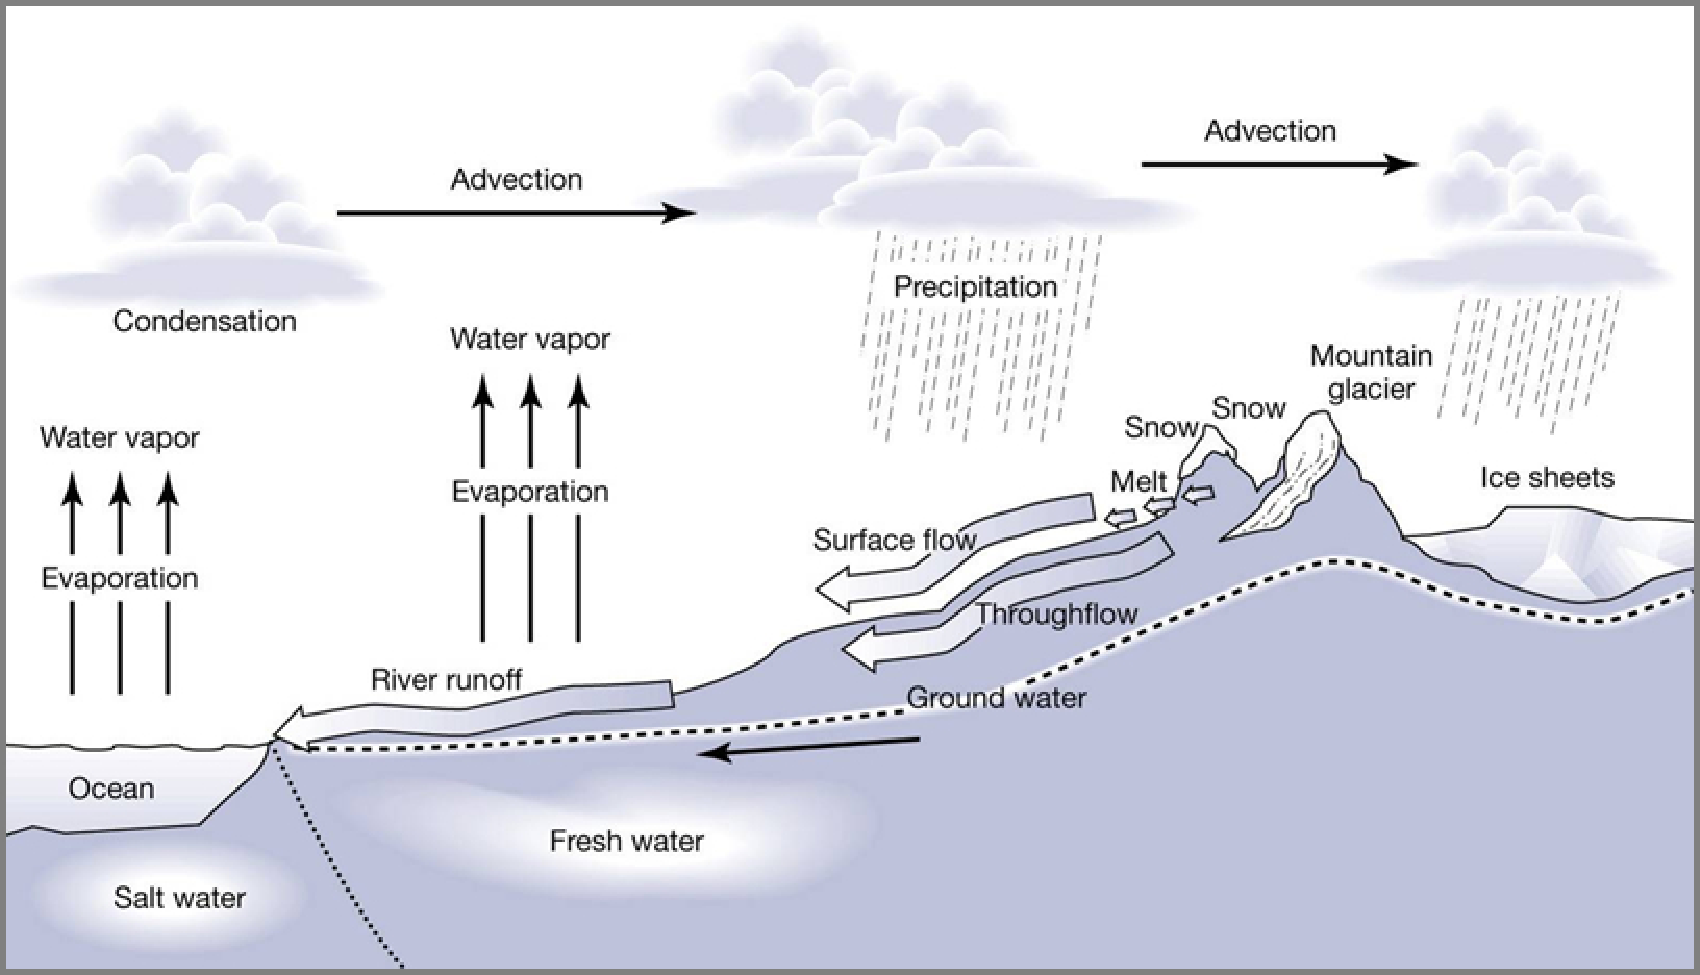
\includegraphics[width=4in]{./globalwatercycle}
\caption{Schematic of the global water cycle.}
\end{center}
\label{fig:globalwatercycle}
\end{figure}

The global water cycle has six major reservoirs. These include the oceans, the atmosphere (split into two reservoirs, one over land and one over the oceans), surface water (including water in lakes, streams, and the water held in the soil), groundwater (water held in the pore spaces of rocks below the surface), and snow and ice. Soil water can be considered separate from the deeper groundwater because soil water occurs in a very thin veneer (around a meter thick) at the surface and can be filled or depleted much faster than the deeper reservoirs of groundwater. As shown in Table \ref{table:inventory}, there is a huge disparity in the size of these reservoirs --- this is one of the important features of the global water cycle that affects its behavior over time.

\begin{table}[h]
\caption{Inventory of water in Earth's reservoirs. The total amount of water is 1,385,990.5 $\times 10^{15}$ kg.\hspace{5cm}}
\begin{tabular}{l c c}\\
\hline
Reservoir & Mass of water in $10^{15}$ kg & Approximate \%\\
\hline
Oceans & 1,350,000 & 97.4\\
Marine atmosphere & 11 & 0.0008\\
Land atmosphere & 4.5 & 0.0003\\
Surface Water & 275 & 0.02\\
groundwater & 8,200 & 0.59\\
Snow \& Ice & 27,500 & 1.98\\
\hline
\end{tabular}\\\\\\
Data from: Chahine, 1992, The hydrological cycle and its influence on climate, Nature, v. 359, p. 373-380; 
Gleick, P.H., 1993, Water in Crisis, Oxford Univ Press, N.Y.
\label{table:inventory}
\end{table}

It should be emphasized that these are all estimates, with varying degrees of confidence. The amount of water in the oceans and the atmosphere are fairly well-constrained; the amount of surface water is less well-constrained because of uncertainties in the soil water; groundwater is even less well-known; the amount of snow and ice is better constrained since it is dominated by Antarctica and Greenland, whose ice volumes can be estimated fairly well. 

Water moves through these reservoirs by a variety of processes. The major processes, along with the amount of water transferred per unit time, are shown in Table \ref{table:estimatedflows}. These estimates have been slightly adjusted from the published literature in order to create a steady state model of the water cycle. One thing that should be noted at this point is that there is a huge disparity in the flow values; we will later see that this has some very important consequences for the dynamics of the water cycle. Before proceeding, it will be helpful to discuss briefly the processes involved in this cycle.

\begin{table}[h]
\caption{Estimated flows of water in the global carbon cycle.\hspace{15cm}}
\begin{tabular}{lc}\\
\hline
Process & Flow ($10^{15}$ kg/yr)\\
\hline
Evaporation from oceans & 435 \\
Evaporation from land (mainly from soil water) & 71\\
Precipitation on oceans & 398\\
Transfer (advection) from marine to land atmosphere & 37 \\
Precipitation (rain) on land & 107\\
Precipitation (snow) on land & 1\\
Meltwater return to surface water & 1\\
Surface runoff to oceans & 34\\
Surface percolation into groundwater & 2\\
Groundwater flow into oceans & 2\\
\hline
\end{tabular}\\\\\\
Data modified from Chahine, 1992, and Gleick, P.H., 1993, to create a steady state model.
\label{table:estimatedflows}
\end{table}

\section{Water cycle processes}
\subsection{Evaporation}
Evaporation from the oceans occurs when water molecules at the ocean surface get enough kinetic energy (energy of motion) to leave the water and enter the atmosphere. Since kinetic energy is gained by the absorption of thermal energy, evaporation will tend to occur more readily at higher temperatures. Equally important, however, is the amount of water already in the vapor form in the atmosphere just above the water surface; evaporation occurs much more readily when the air is very dry, which is the same as saying that it has a low vapor pressure. Wind speed is also important; for instance, clothes hanging on a line dry more rapidly in a good breeze. The breeze tends to bring dry air into closer contact with the clothes, thus helping to maintain a strong gradient in the vapor pressure, encouraging evaporation to occur more rapidly. With no breeze, the air right next to the clothes will acquire a higher vapor content than the surrounding air because of some evaporation from the clothes,; this decreases the gradient of vapor pressure and slows evaporation.

On land, most of the evaporation is actually brought about by plants, who extract moisture from the soil and transpire it through their leaves into the atmosphere. So, this rate is dependent on things like how much soil water is available and how vigorous the plants are growing. This in turn depends on things like the types and numbers of plants and the season. It is reasonable to assume that in most cases, higher temperatures mean higher rates of evaporation, provided that there is enough soil water available. Of course, evaporation from lakes and streams occurs by the same processes described above for the oceans.

\subsection{Advection}
The process of advection transfers water from the atmosphere above the oceans to the atmosphere above the land. This occurs through the circulation of air masses. The magnitude of this flow is constantly changing as weather patterns change, but it can also be affected by such things as the positions of the continents, changes in ocean currents (which can change where evaporation occurs in the oceans), and the locations and elevations of mountains.

\subsection{Precipitation}
Precipitation returns atmospheric water back to the surface in the form of rain and snow. As we all know from personal experience, the timing and magnitude of precipitation is quite variable. For precipitation to occur, condensation must occur first; water vapor must be converted to its liquid or solid form and both of these changes involve a release of heat as mentioned above. Condensation is dependent on a number of factors, but in general, it occurs when and where air that is saturated with water vapor is cooled, provided that there are tiny particles for the water to condense onto. These particles are called cloud condensation nuclei and can be dust or tiny salt crystals or a range of other atmospheric aerosols. The cooling can occur either by rising and expanding or when an air mass comes into contact with some cooler material. Once enough condensation occurs, the droplets may join together, forming big enough droplets to fall down to the surface as precipitation.

\subsection{Snow and ice formation}
Snow falling on the surface in the area of a glacier or large ice sheet accumulates and undergoes a change from snow to solid ice as it gets buried by more and more snow. The magnitude of this flow is assumed to be proportional to the land surface area covered by glaciers.

\subsection{Streamflow}
Streams and rivers throughout the world transport water from the land surface to the oceans. Some portion of the water involved in this process enters the streams from surface runoff during storm events; the rest of the water comes from soil water (or very shallow groundwater) that seeps into stream beds. This flow is unquestionably the easiest one to measure because you can make measurements at the mouths of major rivers. 

\subsection{Percolation}
Liquid water falling on the surface has a number of options; it may fall in a lake or stream or may run off over the surface to a lake or stream, but the majority of it seeps down into the soil where it occupies the pore spaces in the soil. The fraction of this soil water that is not quickly used by plants or lost to a nearby stream seeps further down into the rocks below the soil; in doing so, it enters the groundwater reservoir. On a global scale, this flow is difficult to measure directly, so estimates are derived from looking at the difference between rainfall and other surficial flows of water (streamflow, evapotranspiration).

\subsection{Glacial melting}
Ice in glaciers flows slowly from places of accumulation to the edges, where it may melt or calve into the ocean. At present, most of the ice on Earth is stored in Antarctica and Greenland; when the ice melts in these places, the water produced is added directly to the ocean. This flow is tough to actually measure, but we can infer it based on knowledge that sea level is rising at the present time and assuming that part of that rise is due to glacial melting, while the remaining part is due to warming (thus, expansion) of the surface water.

\subsection{Groundwater discharge}
Groundwater flows, slowly, from higher areas to lower areas. In some cases, it flows back out to the surface as a spring, or into the bed of a river, but these return flows to the surface water reservoir are effectively represented by decreasing the magnitude of the flow from the surface waters to groundwater. Groundwater flows through the pore spaces of loose sediments and sedimentary rocks and thus it is generally confined to following the paths of these layers beneath the surface. Near the margins of continents, these layers eventually come into contact with the oceans and the groundwater slowly seeps out into the oceans. Of all the flows represented in the global water cycle, this last one is probably the least well known and its value is chosen so that the inflow and outflows of the groundwater reservoir are equal, which is necessary for the cycle to be in a steady state (this is not to imply that the system actually is in a steady state --- the opposite is more likely --- but for the purposes of experimentation, it is useful to have a steady state model to serve as a control).

\section{Model Construction}
The basic data for constructing a model of the water cycle is summarized in Tables \ref{table:inventory} and \ref{table:estimatedflows}. This model is relevant for short time periods, measured in years or hundreds of years rather than millions of years, which is why the water that passes in and out of the mantle is ignored here.

\begin{figure}[h]
\begin{center}
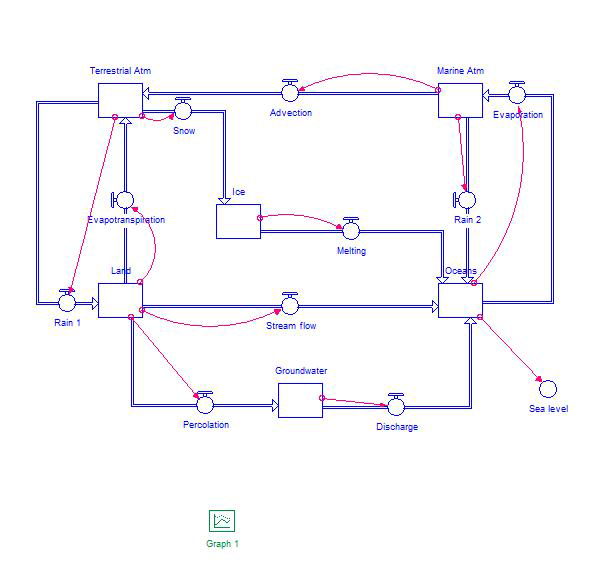
\includegraphics[]{./globalwatermodel}
\label{fig:model}
\caption{Diagram of the global water cycle model.}
\end{center}
\end{figure}

As with the previous modeling exercises, I have given you a starting model (Fig. 2):

\begin{enumerate}
\item The model contains several reservoirs and flows that drain the reservoirs. Each of the flows is a ``draining flow'', and the model is set up so that it is initially in steady-state. This means that if a reservoir has some initial amount that we'll call INIT(Reservoir), and an outflow takes 10 units away during each unit of time, then the outflow is defined as

$$\mbox{Outflow}=10\times\left(\frac{\mbox{Reservoir}}{\mbox{INIT(Reservoir)}}\right),$$

where Reservoir represents the amount in the reservoir at any given time; the quantity in parentheses has units of 1/time and is sometimes called a rate constant or time constant. In this way, if we have more water in the atmosphere, we will have more rain; a very dry atmosphere leads to little rain. Defining the flows in this way is pretty simplistic, and we'll try to define some of these flows in a more realistic manner later on, but as a start, this simple approach will be fine. 


\item The model also includes a converter that monitors sea level over time. Sea level is an important parameter in the global climate system; it is currently rising at a rate of about 10--15 cm/100 yrs. With this monitor, we can see how various changes we will later impose on the steady state model affect the sea level, which will help us gauge the significance of the change. The Sea Level converter is definited according to the following formula:

$$\mbox{Sea\_Level} = 100\times(\mbox{Oceans-INIT(Oceans)})\times \frac{1.0\times 10^{12}}{3.61\times 10^{14}}$$

In this equation, we take the difference between the current amount in the ocean and the initial amount (the initial amount we will say corresponds to a sea level of 0), multiply it by a conversion factor to give us units of cubic meters, then divide by the surface area of the oceans, given in units of square meters. The result is then multiplied by 100 so that the units will be centimeters rather than meters (anticipating that on short timescales such as we will investigate here, most sea level changes will be far less than a meter).

%\item Check to see that the model is in a steady state by running the model while graphing the reservoirs. Steady state in this case means that the amounts in each reservoir do not change over time --- the graph should be a set of straight, horizontal lines. Be sure that in the Time Specs window under the Run menu, you set the DT to 0.01. (Remember that DT is the time step for the calculations; so in this case, the program will calculate the flows of water every 0.01 years, since years are our basic time unit.) If DT is greater than this, the model will behave strangely as it tries to subtract more from some reservoirs than actually exists in those reservoirs. With a small enough DT, the subtractions occur in small enough increments so as not to bankrupt any reservoirs.
\end{enumerate}

\begin{table}[h]
\caption{Reservoir residence times in our model of the global water cycle.\hspace{15cm}}
\begin{tabular}{lc}\\
\hline
Reservoir & Residence time (years)\\
\hline
Ice & 27500\\
Groundwater & 4100\\
Oceans & 3110\\
Land (surface water) & 2.57\\
Terrestrial atmosphere & 0.042\\
Marine atmosphere & 0.025\\
\hline
\end{tabular}
\label{table:residencetimes}
\end{table}

Here is a good opportunity to revisit the concept of the residence time of material in a reservoir; this was first described in an earlier section. Consider the marine atmosphere water reservoir --- it has about $11\times 10^{15}\mbox{ kg}$ of water, and every year, $434\times 10^{15}\mbox{ kg}$ of water are added and subtracted. The residence time is defined as the amount in a reservoir divided by the amount added (or subtracted; they're the same in the steady state). So for the marine atmosphere, the residence time is 0.025 years, or 9.2 days --- a pretty fast turnover time. This is the average amount of time that a given water molecule might spend in the atmosphere. Table \ref{table:residencetimes} below summarizes the residence times of reservoirs in our model. As you can see, one of the striking characteristics of the global hydrologic cycle is the huge range in residence times; this turns out to be important in understanding how this cycle responds to changes.




\section{Human impacts on the water cycle}
Human activities affect the water cycle in a number of ways, reflecting the great importance of water in our lives. Our withdrawal of groundwater, our storage of water in reservoirs, our diversion of surface water for irrigation, and our land-clearing, wet-lands filling, and vegetation burning (burning plant material releases water vapor) all represent modifications to the global water cycle. Figure 3 shows how the total amount of water used by humans is broken down according to use; it also shows how this use has changed over time, including how per capita use has changed. This figure shows that agricultural uses greatly outstrip other water uses. A very important aspect of these data is the pattern of water use over time; it follows an exponential curve. This is a troubling sign that tells us our current use of fresh water is not sustainable; changes will have to be made. The use of water varies geographically and economically, as can be seen in the Table \ref{table:wateruse}, which helps to put our water use into the proper global perspective. Our world in data also has some great, more up-to-date graphics: \url{https://ourworldindata.org/water-use-stress}.

\begin{figure}[h]
\begin{center}
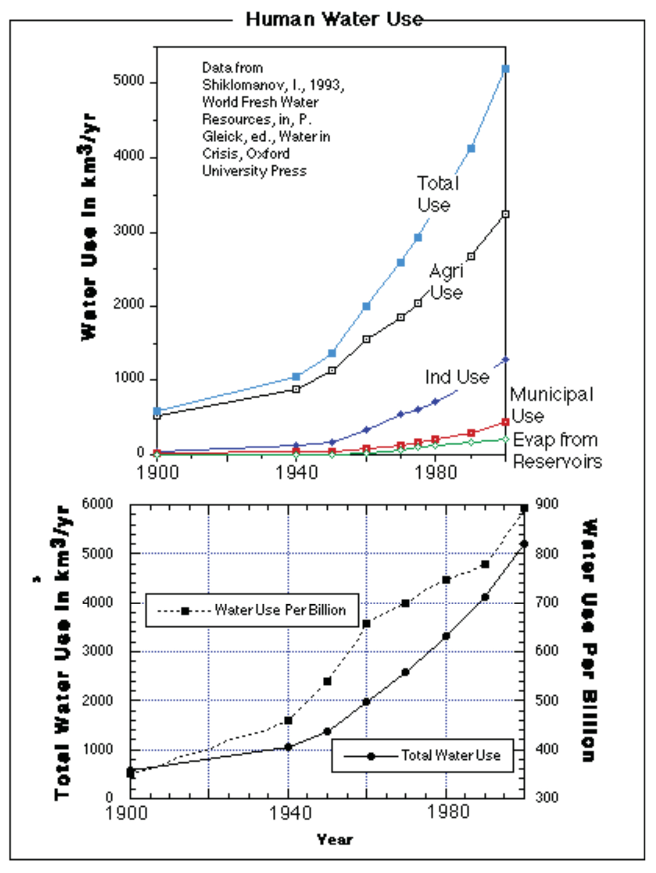
\includegraphics[width=3in]{./wateruse}
\label{fig:wateruse}
\caption{Human water use during the 20$^{\mbox{th}}$ century.}
\end{center}
\end{figure}

\begin{table}[h]
\caption{Per capita water use in 1987.\hspace{15cm}}
\begin{tabular}{l c c}\\
\hline
Region & m$^3$/yr & gallons/day\\
\hline
Africa & 244 & 176\\
South America & 476 & 344\\
Asia & 526 & 380\\
Europe & 726 & 525\\
U.S.A. & 2161 & 1563\\
World & 660 & 477\\
\hline
\end{tabular}
\label{table:wateruse}
\end{table}

In the series of experiments outlined below, we will investigate the effects of some of the more significant of these human modifications to the global water cycle, first separately, and then together.

\subsection{Groundwater mining}
The first question we will investigate concerns the effect of our withdrawal of groundwater on the behavior of this system. At present, it is estimated that about $2\times{10}^{14}\mbox{ kg}$ of groundwater are withdrawn each year around the globe. This works out to be about 25 gallons/person/day. Americans are responsible for an average of 400 gallons/person/day. You may protest and say that this number is way too high, but this number is not the amount that you as an individual may use in your house every day. But our food and most of the material goods that surround us require the use of water and this amount is much greater than the average individual uses within the home (see Municipal Use curve in Figure 3). The point here is that we have to think of ourselves not as separate, isolated individuals, but rather as parts of a much larger, complex society that collectively consumes vast quantities of water as well as other resources.

As it turns out, about 70\% of this groundwater withdrawal occurs in places where there is relatively little rainfall at present, which means that the groundwater in these areas in not being recharged at the present time. In the past, under a different climate, these areas received more rainfall, allowing for the accumulation of groundwater, but at the present, our withdrawal amounts to groundwater mining --- it is not being replenished.

To do this experiment, we need to modify the original model in order to represent this withdrawal. Clearly, we need to add a flow that drains the groundwater reservoir, but where should that flow go to? Should it empty out into the oceans, into the surface water reservoir, or into the atmosphere above the land? This raises the question of what happens to water that is removed by wells that tap into the groundwater? Most of the water is either used in homes, industry, or irrigation; in other words, it enters the realm of the surface water (land) reservoir. So, we need to add a new flow that goes from the groundwater reservoir and ends up in the surface water (land) reservoir. From there, it can either run off over the surface, it can be evaporated, or it can seep back down into the groundwater. Add this new flow and label it Withdrawal. 

The next question is: how to define this new flow? Is it proportional to the amount of water stored in the ground, is it constant over time and independent from any other variables? Initially, let's explore a very simple case, one where the withdrawal flow is defined as a constant, with a value of 0.2 since our basic unit of water is $10^{15}\mbox{ kg}$ and the estimated magnitude of this flow is $2\times 10^{14}\mbox{ kg/yr}$. We can also make it so that there is a limit on how much can be withdrawn by setting the groundwater reservoir as a non-negative reservoir; this is done by double-clicking on the groundwater reservoir and making sure the non-negative box is checked.

Before running the model, let's try to make some predictions --- at least concerning the general behavior of the system. If we run the model for 100 years (with a time step of 0.02), we would remove 20 units (1 unit = $10^{15}\mbox{ kg}$) of water from the groundwater reservoir and that amount would be added to the surface water (land) reservoir. But, where will this water go once it gets into the land reservoir? If it all ran off to the oceans, there would be 2 extra units of water added there, which would result in a sea level rise of 5.5 cm in 100 years. But surely not all of the water will go straight to the oceans, so the 5.5 cm rise could be considered a maximum. In making predictions, it is good to think about more than just the details --- we should try to figure out how the system as a whole will respond to this change. Will it find a new steady state or not? If so, what will be the characteristics of that steady state? Which reservoirs are likely to increase and which are likely to decrease?

When you run this model (for 100 years with a time step of 0.02, using the Runge-Kutta-2 integration method), it would be a good idea to plot the values of all the reservoirs and then do some accounting, figuring how much was lost by which reservoirs, and then how much was gained by the other reservoirs. Does the groundwater reservoir actually decline by the full 20 units of water that were withdrawn? If not, you should try to explain why this has happened. In considering the question of whether or not the system stabilizes again, you should think about how much time you might need for some of the reservoirs to respond to the changes you've made. You may find it useful to apply the concept of a response time here. The response time is defined as time needed for 67\% of the eventual change to occur as a reservoir goes from some altered condition to a steady state. If we think of a simple
case where a reservoir, $W$, is drained by one flow, $F$, and if that flow is defined as

$$F=kW,$$

where $k$ is the steady-state flow divided by the initial amount in the reservoir, then the response time is $1/k$. In the case of the groundwater reservoir, $k=\frac{2}{8200}\mbox{ yr}^{-1}$ and so the response time is 4100 yr.

In reality, the response time will be slightly less than this value since this is not an isolated reservoir; it has connections to the rest of the system. The main point is that this is a very long response time and we cannot expect to see this reservoir approach its new steady state in 100 years. Looking at the above equation, we can see that if the initial value of the groundwater reservoir were greatly reduced, to a value of 100, the response time would be greatly reduced and we would therefore expect to see a new steady state condition by the end of our simulation. Although modifying the system in this way represents a deviation from reality, we can learn some valuable things about the general behavior of this system through this experiment, so it is a worthwhile one to pursue. This experiment is easy to set up; simply change the initial amount in the groundwater reservoir and make sure that the discharge flow is also modified, though this is done automatically if you have defined the discharge flow as:

$$\mbox{Discharge} = 2\times\left(\frac{\mbox{Groundwater}}{\mbox{INIT(Groundwater)}}\right).$$

The results of this experiment, compared with the original experiment, lead to a number of good questions. Although we have withdrawn the same amount of water, the sea level rise is far less and the total reduction in the groundwater reservoir is also far less. Why has this happened? Once you have finished experimenting with the effects of groundwater withdrawal, you can effectively disable the added flow by setting it to zero; in this way, it can be revived later when we combine the various effects of human water use.

\subsection{Irrigation by diverting surface water}
Although some of the groundwater withdrawal is used for irrigation, it turns out that around the world, the vast majority of water used for irrigation comes from surface water that is diverted into fields. A number of recent estimates put the total amount of water used for this purpose at about 2600 km$^3$ every year --- this is equal to 2.6 units of water in our model. Some of this diverted water flows through the fields without being absorbed, but much of it soaks into the soil and is either evaporated and transpired or it seeps into the groundwater.

How can we change the model to represent the effects of this diversion? One simple way of doing it is to simply decrease the stream flow by an amount equal to the water diverted for use in irrigation. This makes sense if you think about a river like the Colorado; a great deal of the Colorado's water is diverted (mainly into California) and the result is that the stream flow, as measured at the point where the Colorado empties into the ocean is now reduced to almost nothing. So if we redefine the stream flow in our model to

$$\mbox{stream\_flow} = 34\times\left(\frac{\mbox{Land}}{\mbox{INIT(Land)}}\right)-2.6,$$

we will have incorporated this aspect of human water use and we can then run a simple experiment in which we keep this amount steady and examine the response of the system over 100 years. As always, try to predict how the system will respond before actually running the model. After running the model, it might be useful to summarize the losses and gains of the various reservoirs after 100 years of elapsed time.

Once you have finished experimenting with the effects of surface water diversion, you can effectively disable it by changing the 2.6 in the equation above to zero. We will revive this effect later when we combine the various effects of human water use.

\subsection{The effects of reservoirs (held back by dams)}
Over the past 60 years or so, there has been an explosion in dam-building around the world; this has led to the creation and filling of reservoirs that effectively add to the surface water. As the reservoirs fill with water, the amount of stream flow going to the oceans is decreased, but it should return to normal after filling. How much do reservoirs add to the surface water? As of 1994, the total volume of these reservoirs is estimated to be 5,000 km$^3$, which is equivalent to $5\times{10}^{15}$ kg of water --- 5 units of water in our model. It is estimated that by the end of the century, the volume of reservoirs could rise to as much as 7,500 km$^3$ if developing nations have enough money. Of course, as time goes by, the reservoirs will fill with sediment and this volume will decrease, but to begin with, let's model the simple case where we assume no sedimentation.

Our task now is to figure out a good way to represent this change to our model. Perhaps the simplest way is to mimic what a dam does --- it creates a new space for storing water and then temporarily reduces the flow of water until the reservoir is filled, then stream flow returns to normal. In our model, this will mean that we reduce the stream flow that transfers water from the Land reservoir to the Oceans and redirect this withheld water into a new reservoir, called Reservoirs (what else?) until it has accumulated 5 units of water; then stream flow returns to normal. We will also want to make sure that any excess from Reservoirs is sent back into the Land reservoir. But water in reservoirs doesn't just accumulate there --- some of it is evaporated and some of it seeps into the ground. It is estimated that about 5\% of the water seeps into the ground each year and another 3.5\% is evaporated each year --- both of these rates are higher than those for the globally averaged surface water and this is the main reason for treating the water held behind dams as a separate reservoir. Furthermore, our scheme will assume that all reservoirs are built at the same time and will attempt to fill the reservoirs in 10 years; this means that we will try to reduce the runoff flow by 0.5 units each year.

To make these changes, we need quite a few new additions to the model, as shown in the diagram below.

\begin{figure}[h]
\begin{center}
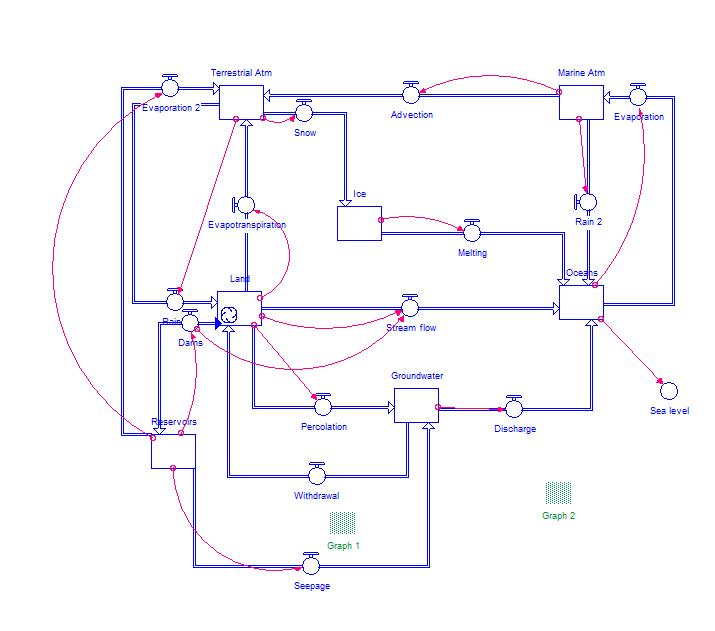
\includegraphics[]{./dammodel}
\label{fig:dammodel}
\caption{Diagram of the model after incorporating dams.}
\end{center}
\end{figure}

In your model, double-click on Dams, click on the Bi-Flow box in the upper part of the window and then define it as follows:

$$\mbox{Dams} = \mbox{if (Reservoirs}<\mbox{5) then 0.5 else (Reservoirs-5)}.$$

Here we see a useful feature of the program --- the ability to make a parameter dependent upon some condition through the use of an if-then-else statement that will be familiar to anyone with experience writing computer programs. This statement instructs the program to constantly be checking the amount of water in Reservoirs. If that value is less than the amount to be held by all the reservoirs (5 units) then Dams will be assigned a value of 0.5 units per year. But if the amount of water in Reservoirs is equal to or greater than this targeted amount, the Dams flow is defined as the difference between the two, which could be a negative number (this possibility may arise later when we modify the model).

Next, modify the Stream Flow to incorporate the Dams converter as follows: 

$$\mbox{Stream flow}=34\times\left(\frac{\mbox{Land}}{\mbox{INIT(Land)}}\right)-\mbox{Dams}$$

In this way, Stream Flow is reduced when the value of Dams is greater than 0; it will be unchanged when the value of Dams is 0, and greater than normal when the value of Dams is less than 0.

The next step is to add two new outflows to Reservoirs. One of these flows will be called Seepage and the other will be called Evaporation 2 (since we already have 2 other evaporation flows we use a number in the name to distinguish it); these new flows will be defined as:

$$\mbox{Seepage} = 0.05\times\mbox{Reservoirs}$$
$$\mbox{Evaporation\_2} = 0.035\times\mbox{Reservoirs}$$ 

Note that we have set this up with the idea that the reservoirs will fill in 10 years. Do you think that will really happen? We should consider what really occurs when a reservoir fills in; some of the water held back is evaporated, and some of it sinks into the ground, slowing the rate of filling --- this is like trying to fill up a bucket with a few holes in it. Our modified model will adjust to these losses since it will continue the filling until the reservoirs have filled up regardless of how ``leaky'' the reservoirs may be.

As always, try to predict how the system will respond before actually running the model. How much water do you think will end up being withheld from the oceans as a result of filling the reservoirs with 5 units of water? Will the system return to a steady state? If so, how long will it take? Will sea level drop by more or less than the 1.38 cm expected by taking 5,000 km$^3$ and spreading it out over the $3.61\times 10^{14}\mbox{ m}^2$ surface area of the oceans? As before, it will be useful to summarize the losses and gains of the various reservoirs after 100 years of elapsed time.

A refinement to this model would be to include reservoir sedimentation. The accumulation of sediment in reservoirs fills them up, thus reducing the volume of water they can hold. This is an especially big problem on rivers with high sediment loads like the Yellow River in China, where reservoirs may have useful lifetimes of less than a few decades. We can easily incorporate this effect into the model by first adding a new converter called Reservoir Volume. Set this new converter equal to Time and then click the Become graph button to make Reservoir Volume vary over time. Draw the graph such that the volume stays at 5 for the first 30 years, and then declines steadily to a value of 2.5 by 100 years (here we are assuming a 200-year lifetime for most reservoirs). Next, draw a connector arrows from Reservoir Volume to the Dams flow. Redefine this flow in the following manner:

$$\mbox{Dams}=\mbox{if}(\mbox{Reservoirs}<\mbox{Reservoir volume})\mbox{ then }(0.5)\mbox{ else }(\mbox{Reservoirs}-\mbox{Reservoir volume})$$

How do you think this change will affect the system? Make your predictions, run the model and then compare it with the previous model in which no sedimentation occurs. After completing this experiment, don't remove these additions that represent the filling of reservoirs; we will use this model in the next experiment.

\subsection{Cumulative effect of human modifications of the water cycle}
Now let's combine the changes we made in the previous three experiments in order to investigate the net effect of our use of water resources. This is an easy experiment to set up since we've already gone through the procedures for modifying the model to represent the various human-related modifications. For the sake of simplicity, make the Reservoir Volume graph stay steady at 5 over the 100 years of the experiment. In doing this, we assume that continued dam-building will offset reservoir volume lost to sedimentation.

Before running the model consider the following question: Will the combined effect be the same as simply adding up the results of the separate experiments? This is clearly a very difficult question and we can only make a guess without running the model. As you look at the results of this combination experiment, you should see that after the reservoirs held back by dams fill entirely, the system behaves differently and most system components change in a nearly steady or linear manner over at least the 75 years following the filling. This means that we can calculate a rate of sea level fall that describes the behavior of the system during this time period. This rate of sea level fall is then what we would expect at the present time if we considered that we have passed the big dam-building phase of our development. The calculated rate turns out to be about 0.2 cm/yr or 2 mm/yr.

How do our results compare with the observations of sea level? According to the best estimates, sea level is actually rising at a rate of about 1--2 mm/yr. What does this mean? Are our assumptions used in the model incorrect? Are the basic data used in our model incorrect? Or are there other processes contributing to sea level rise that we have ignored in our model? The basic logic used to represent the human modifications to the water cycle are not likely to be the culprits. The data used would have to be off by a factor of 10 or more, and that also seem unlikely. Instead, the best explanation is probably that we are missing some process in our model, or we have not represented some processes that are in fact causing sea level to change in the opposite direction from our model results. So, what could we be missing? 

One thing that certainly contributes to sea level rise is the expansion of water that occurs when water is heated. It is now well-established that the earth has been warming in the past 100 years and that means that the surface of the oceans must also be warming, thus causing expansion of the water and a rise in sea level. This expansion should, given the recent warming, cause a sea level rise at a rate of about 4 cm per 100 yrs or 0.4 mm/yr. Another observation that is linked to global warming is that glaciers around the world are shrinking -- they are not in a steady state. This means that the flow from Ice to Land in our model should exceed the inflow into the Ice reservoir. Estimates of how much glaciers and ice sheets are very poorly constrained --- this is a difficult thing to measure. The best estimates for ice melting translate into a sea level rise of about 7 cm/100 years or 0.7 mm/yr. It is important to note, however, that this estimate is most strongly affected by what goes on in Alaska, Greenland, and Antarctica, where most of the ice is stored, and very little is known about the rate of change of this ice mass over recent times. At any rate, the recent global warming should produce a sea level rise of around 1.1 mm/yr. In fact, sea level appears to have risen by about 12--15 cm in the last 100 years --- a rate of 1.2 to 1.5 mm/yr --- in pretty good agreement with the estimates from water expansion and ice melting.

So, we have a problem on our hands. Human use should lead to a rate of sea level fall of about 2 mm/yr, while warming should lead to a sea level rise of about 1.1 mm/yr, so the net change should be about 0.9 mm/yr of sea level fall. Instead, we see a rise of about 1.2 to 1.5 mm/yr. These modeling experiments suggest that it might be a good idea to scrutinize the estimates for sea level changes due to ice melting and ocean warming. On the other hand, this discrepancy might be telling us that our understanding of the global water cycle is leading us to overestimate the effect of human water use on the global system --- the implication would be that despite all of our uses, we are not having any net effect on sea level.

Our experiments have shown that we must take human modification of the global water cycle seriously; we are having a significant effect. Of course, we should not lose sight of the reality that most of the major threats from water use come at more local and regional levels, where usable groundwater and surface water provide the ultimate limitations on human occupancy.

\end{document}
\subsection{Altering the weather}
In our standard model, 37 units of water are transferred from the marine atmosphere to the terrestrial atmosphere each year. This represents the average effect of global weather patterns; on shorter time scales, this rate is much more variable. In this experiment, we ask the question: What would happen if weather patterns changed so that more water vapor was transported from the marine atmosphere to the terrestrial atmosphere? What could cause a change like this for a long enough period of time that we might see some global effects? One possible mechanism is the El Nino-Southern Oscillation. This change in the location of the warm water in the equatorial Pacific appears to alter the global climate and one way it affects global climate is by changing where water vapor enters the atmosphere; this could cause a change in the average advection from the oceans to the land. Another possibility is a change in ocean currents, such as when the Isthmus of Panama closed off (about 3 million years ago). This stopped the westward flow of warm, tropical waters and this water was instead redirected up to the north, forming the Gulf Stream. Something like this could conceivably have changed the ratio of precipitation on land to sea. Consider a 10\% increase and a 10\% decrease. In this experiment, be sure to explain how you made the change to the model and be careful and thorough in your analysis of how the model responds. For instance, pay close attention to what happens in the first few years of this experiment and refer back to the table listing the residence times for the reservoirs in this model.

What changes need to be made in the model in order to carry out these experiments? There are several ways of doing this, but one way is to add a converter called Advection Change, make it equal to 1.1 or 0.9 and multiply it by the Advection equation, as shown below, to produce a 10\% increase or decrease. An alternative method is to make Advection Change a graphical function of time so that the 10\% change would occur shortly after the beginning of each run --- this has the advantage of letting you see that the system is in a steady state before the change occurs. The graph can be set up as shown below; the key here is to make it a segmented graph with instantaneous jumps --- this is done by clicking on the button at the lower left of the graph window.

As always, try to make some predictions about how the system will respond to this change. Will these experiments turn out to be mirror images of each other? What will happen to the marine and terrestrial atmospheres? Will they continue to decline indefinitely, or will they arrive at a new steady state? If they do settle down, how long will it take? How will the rest of the system react to this change? One thing to keep in mind is that if you are trying to understand why a reservoir has changed in a certain way, it is often helpful to look at all of the inflows and outflows in the form of a graph.

\subsubsection{Refining the model}
Now, we'll try to make some refinements to the model. Our previous description of the process of evaporation was awfully simple and doesn't really do a good job of capturing the essence of the process. For instance, the amount of evaporation from the oceans is not really a function of the total mass of water in the ocean. Instead, it should be the product of the surface area of the ocean times a rate in cm/yr and that rate should depend on things like wind velocity and the water temperature and the relative humidity at the sea-air interface. At this point, we may decide to incorporate a detailed set of equations for evaporation, or we may decide to incorporate a simpler version that nonetheless represents one of the important aspects of evaporation, namely, that it is dependent on the temperature.

Here, we will take a simple approach and understand that our model results will be meaningful only in a qualitative sense. Our goal then is to redefine the evaporation flows so that they are dependent on the global temperature; evapotranspiration from the Land will also be dependent on how much water is available since in many areas, the amount of water is the limiting factor in determining how much evaporation occurs.

First, we need to represent the global temperature in our model. Global temperature is really determined by the solar energy system, which is modeled in another section. We could import the model that we developed previously and make connections between it and the global water cycle, but at this point, we will adopt a simpler approach. Since water is the most important greenhouse gas, we can make a simple addition to our model that relates the total atmospheric water vapor to the global temperature. Before forging ahead, we should hesitate to think a bit more about what we are doing to our model. More water vapor will lead to a warmer Earth, which will then lead to more evaporation, thus setting up a positive feedback mechanism. On the other hand, water vapor condenses to form clouds, which block solar radiation from the surface, reflecting it back to outer space, thus cooling the Earth, setting up a negative feedback mechanism that will tend to counteract any warming or cooling trend. What is the net effect of water? This is the matter of some current debate, but some satellite measurements (Chahine, 1992) indicate a slight net warming effect. In the face of this uncertainty, we'll go ahead and model both possibilities.

\subsubsection{Modifying the Model in 6 Steps}
\begin{enumerate}
\item The first step in modifying the model is to place two new converters in your model, near the atmosphere reservoirs; label one of them Total Atmos and the other Global Temp. Connect both atmosphere reservoirs to Total Atmos and define it as the sum of the two. Now, make an arrow connecting Total Atmos to Global Temp, define Global Temp as being equal to Total Atmos, then hit the Become Graph button and define the graph as shown below. The reasoning behind the graph is pretty simple, and here it is: Earth's greenhouse effect raises the temperature by $33^\circ$C; half of that warming is due to water vapor, so without any water vapor, the Earth would be $16.5^\circ$C cooler. As the concentration of a greenhouse gas grows, its contribution to the greenhouse tends to increase by smaller and smaller amounts. With this in mind, we will estimate that with twice as much water in the atmosphere, the Earth would be $5^\circ$C warmer. Figure \ref{fig:modifymodel1} uses these three control points and the assumption that the actual form of this curve is probably smooth.

\item The next step is to define a new converter called Temp Feedback that will determine how much to change the various flows given a certain temperature increase relative to the starting temperature of $15^\circ$C. We will set this up in such a way that we can easily modify it; this will require two additional converters, set up as shown in Figure \ref{fig:modifymodel2}.

Later, we will explore the effect of changing $n$ from 1 to 2, but for now, simply define it as being equal to 1. Kick will be set up as a graphical function of time; double click on it and set it equal to time, then hit the Become Graph button and make Kick have a value of 0 for the whole time. Set the range of time from 0 to 10 (we will only modify kick during a very brief time at the beginning of the experiment). Now the question is how to defined Temp Feedback. The plan will be to use this feedback factor to multiply by the various flows that are likely to be temperature sensitive. One way to define this factor is as follows:

$$\mbox{Temp Feedback} = \mbox{if (Global Temp}\>0\mbox{) then}\left(\frac{\mbox{Global Temp + Kick}}{15}\right)^n\mbox{ else 0}.$$

An if-then-else statement is used here because the program has difficulty if the global Temp becomes negative and $n$ has a value between 1 and 2. Note that if the temperature does drop below 0, the system will effectively shut down since we will multiply Temp Feedback by several of the major flows in this system.

\item The next step is to change the way we define the two evaporation flows so that they respond to changes in the global temperature. In addition, we will alter the evaporation coming from the oceans so that it is not dependent upon the amount of water in the oceans. To make these changes, first add connector arrows going from Temp Feedback to the two evaporation flows, then remove, (using the dynamite) the connector going from Oceans to Evap. Then double-click on each of the evaporation flows and redefine them as follows:

$$\mbox{Evap = 435 * Temp Feedback}$$

$$\mbox{Evapo Trans} = \mbox{Land}*\left(\frac{71}{\mbox{INIT(Land)}}\right)*\mbox{ Temp Feedback}.$$

This way of incorporating the temperature into the evaporation flows is set up so that a doubling of the temperature would lead to a doubling of evaporation. It is very important that the Global Temp graph be defined so that the initial temperature is 15. These new changes are shown in the Figure \ref{fig:modifymodel3}.

\item Evaporation is not the only process to be affected by a change in the temperature, so we must find ways of incorporating a temperature dependence into some of the other flows. The melting of ice is an obvious candidate that is likely to be very sensitive to warming; to modify the Melting flow, draw a connector arrow from Temp Feedback to Melting and redefine melting as follows:

$$\mbox{Melting }=\mbox{ Ice}*\left(\frac{1}{\mbox{INIT(Ice)}}\right)*(\mbox{Temp Feedback})^2$$

By squaring the Temp Feedback, we are effectively making this flow more sensitive to warming than the other flows. If the Earth grows warmer the amount of precipitation falling in the regions of ice should decrease. As this form of precipitation changes, so must the amount going to the Land reservoir. This means that we need to overhaul the way we determine precipitation from the terrestrial atmosphere.

\item We'll start to modify the precipitation flows by creating another new converter, placed near the Terrestrial Atm reservoir and call it Total Precip and define it as follows:

$$\mbox{Total Precip }=\mbox{ Terrestrial Atm}*\left(\frac{108}{\mbox{INIT(Terrestrial Atm)}}\right)$$

This will simplify our formulations for the Rain and Snow flows, which should be
rewritten as:

$$\mbox{Snow }=\left(\frac{\mbox{Total Precip}*\left(\frac{1}{108}\right)}{\mbox{Temp Feedback}}\right)$$

$$\mbox{Rain 1}=\mbox{Total Precip}-\mbox{Snow}$$

This way if the temperature increases, the Temp Feedback, which is initially equal to
1, increases, thus decreasing Snow and the amount falling as rain adjusts to make up
the difference between Snow and the Total Precip.

\item The final flow to alter will be Stream Flow. This is not such an obvious flow to change, but we need to modify it so that it reflects the reality that the land surface in many areas has a finite capacity for absorbing and holding water. This can be seen on a smaller scale during a heavy rainfall; the soil absorbs the rain water for a while, but then it's carrying capacity is met and additional rain flows over the surface, and heads towards a stream. So, as the holding capacity is approached, the rate of water leaving the scene increases. If we extend this analogy to our whole Land reservoir, it means that we want to modify it so that as more water accumulates, it flows out of the reservoir at a greater and greater percentage of the amount of water in the reservoir. One way of doing this is

$$\mbox{Stream Flow}=34*\left(\frac{\mbox{Land}}{\mbox{INIT(Land)}}\right)^2.$$

Now that we have changed just about all of our flows, we are ready to check for the
steady state and then experiment. Before proceeding, we should review the changes
we've made. Figure \ref{fig:modifiedmodel} shows the modified model in which the gray-toned elements are the unchanged ones and the ones in black are those we have changed.
\end{enumerate}

Before beginning with the experiments, make sure that your model is in a steady state. If you have difficulties achieving steady state, re-read the above instructions and check all the modified parts of the model.

\subsubsection{Experiments with the modified water cycle model}
\begin{enumerate}
\item What is the effect of a brief warming? First, leave the value $n$ at 1 and then modify the Kick graph so that it has a small jump of 1.0 degrees from time 1 to 2 --- a year-long warming pulse to get the system moving. This graph should be in the discontinuous form --- click on the button in the lower left of the Kick graph window. What do you think will happen? Try to predict how the Global Temperature and sea level will change over time. At first, run the model for 10 years with a time step of 0.02, using the Runge-Kutta 2 integration method. Later, you may want to run the model for longer periods.

\item What is the effect of changing the $n$ value? Use the Sensitivity Specs window to step through different values of $n$, from 1 to 2 in increments of 0.1 to find the value at which the system goes into a sustained warming --- a warming that lasts longer than the Kick.

\item Why does the system behave as it does? The way to approach this problem is through forming a hypothesis and then testing it by studying the key reservoirs and flows. This may require that you run the model a bit longer here. Does this system go into a runaway state or does it settle down eventually? Another thing that might help here is to consider a simpler version of this kind of model and put a positive feedback mechanism in it and observe what happens -- then you might be able to apply what you learn in the simpler model to the more complex one, at least in a general way. Here's an example of what the simpler model may look like.

\item How much of a "kick" is needed to get the system into a state of sustained warming? Use an $n$ value of 1.6, then step through a series of decreasing kicks, starting with 1.0 and going to 0 until you find the critical value.

\item What is the effect of a cooling "kick"? Use an $n$ value of 1.6 and a the smallest possible kick, determined above, only make it negative instead of positive (cooling instead of warming).
\end{enumerate}

\subsubsection{A caveat on the revised model}
We made a large number of changes in this last model to explore the general effect of adding in a temperature sensitivity. Based on what is known about these processes, it makes sense to have them respond to temperature, but the exact way we built this temperature dependence into our model is not based on careful measurements, theory, or observations and so we cannot expect our model to give realistic results in a quantitative sense.

Our inferences from this last model can only be qualitative. What is meant by this? It means that, as we study the results of one of these experiments, we might conclude that with this temperature-sensitivity, the system undergoes rapid change, driven by positive feedback, but there is a limit to this change imposed by all of the other flows that are effectively negative feedbacks. Or we might say that the system responds unevenly to warming and cooling changes; cooling seems to initiate a true runaway behavior taking the system all the way to a frozen state. We cannot place much importance on the rates of change or the magnitudes of change in a numerical sense; for instance, our model shows that the whole system is capable of freezing solid in just a few years, but of course this is not at all realistic. In particular, we have not allowed for the fact that warming of the oceans occurs very slowly compared to the atmosphere, and yet we have the evaporation from the ocean responding to the temperature that is defined solely on the basis of how much water vapor is in the atmosphere. A more realistic version of this temperature dependence can be made by connecting a solar energy system model (the 3-box climate model) to our hydrologic cycle model.

\end{document}
